\documentclass[UTF8]{ctexart}

\usepackage{amsmath}
\usepackage{float}
\usepackage{cases}
\usepackage{cite}
\usepackage{graphicx}
\usepackage[margin=1in]{geometry}
\geometry{a4paper}
\usepackage{fancyhdr}
\usepackage{booktabs}
\pagestyle{fancy}
\fancyhf{}


\title{$KNO_3$溶解热的测定}
\author{522111910161 尚子翔}
\date{\today}
\pagenumbering{arabic}

\begin{document}

\fancyhead[L]{}
\fancyhead[C]{$KNO_3$溶解热的测定}
\fancyfoot[R]{\thepage}

\maketitle
\tableofcontents
\newpage

\section{实验目的}
\begin{enumerate}
    \item 了解热效应测定的基本原理。 
    \item 掌握摩尔积分溶解热、摩尔微分溶解热、摩尔积分稀释热和摩尔微分稀释热的定义。
    \item 使用电热补偿法借助微机控制测定硝酸钾在水中的积分溶解热。
    \item 使用作图法求出硝酸钾在水中的微分溶解热,积分冲淡热和微分冲淡热。
\end{enumerate}



\section{实验原理}
恒温恒压下1mol纯物质溶解于一定量的溶剂中形成溶液时所产生的热效应称为此物质在该条件下的摩尔积分溶解热,用$\Delta_{sol}H_m$表示。摩尔积分溶解热不仅与溶质溶剂的本性有关,而且还与所形成溶液的浓度有关。随着溶液浓度减小,摩尔积分溶解热趋于定值,此值称为该物质的无限稀释摩尔积分溶解热。物质在25℃时以水为溶剂的无限稀释摩尔积分溶解热可从手册中查得。恒温恒压下,在一定量某浓度的溶液中加入$dn_2$量的溶质,产生的热效应$d(\Delta_{sol}H_m)$与$dn_2$之比称为摩尔微分溶解热。由于加入溶质的量为$dn_2$,可以认为溶液的浓度不变。因此,摩尔微分溶解热亦可以认为是在一定浓度的大量溶液中加入1mol溶质所产生的热效应。

恒温恒压下,将一定量溶剂加入到含1mol溶质的溶液中形成较稀溶液时的热效应为摩尔积分稀释热或摩尔积分冲淡热,用$\Delta d_{il}H_m$表示。摩尔积分稀释热为稀释前后溶液的摩尔积分溶解热之差$\Delta d_{il}H_m=\Delta_{sol}H_m(2)-\Delta_{sol}H_m(1)$若加入溶剂的量为$dn_1$,则产生的热效应$d(\Delta_{sol}H_m)$与$dn_1$之比称为摩尔微分稀释热或摩尔微分冲淡热。显然摩尔积分稀释热和摩尔微分稀释热均与所形成溶液的浓度有关。

无机盐类的溶解通常包含晶格的破坏和离子的溶剂化两个过程。前者为吸热过程,后者为放热过程,盐类的溶解热是这两种热效应的总和。测量盐类的溶解热是在绝热式热量计中进行的。本实验测定硝酸钾在水中的溶解热,由于硝酸钾的溶解过程为吸热过程,故根据电热补偿法原理采用NDRH-2S型微机测定溶解热实验系统进行溶解过程热量测定,该系统能自动完成$KNO_3$溶解热实验数据的测量、记录及处理全过程。该系统主要由系统软件和热量测定两部分构成,基本装置如下图所示。

其原理为先测定含有确定量水的绝热体系的起始温度T,在绝热恒压条件下向水中加人一定质量的硝酸钾,随着溶解过程的不断进行,体系的温度不断下降,为了使体系回复到实验前的起始温度需要不断由电热丝加热体系,根据所消耗的电能便可求出溶解过程的热效应$Q=PRE=IVt$式中:1为通过电阻为R的电热丝的电流强度,V为电热丝两端所加的电压,t为通电时间,此Q值即为所加人硝酸钾在此溶解过程中吸收的热量。

根据摩尔据摩尔积分溶解热的定义,硝酸钾的摩尔积分溶解热$\Delta_{sol}H_m=\frac{Q}{KNO_3}$。若定义溶解每摩尔硝酸钾所用水的量$n_0=\frac{n_{H_2O}}{n_{KNO_3}}$则由实验测定不同$n_0$下的$\Delta_{sol}H_m$可作下图。

\begin{figure}[H]
  \centering
  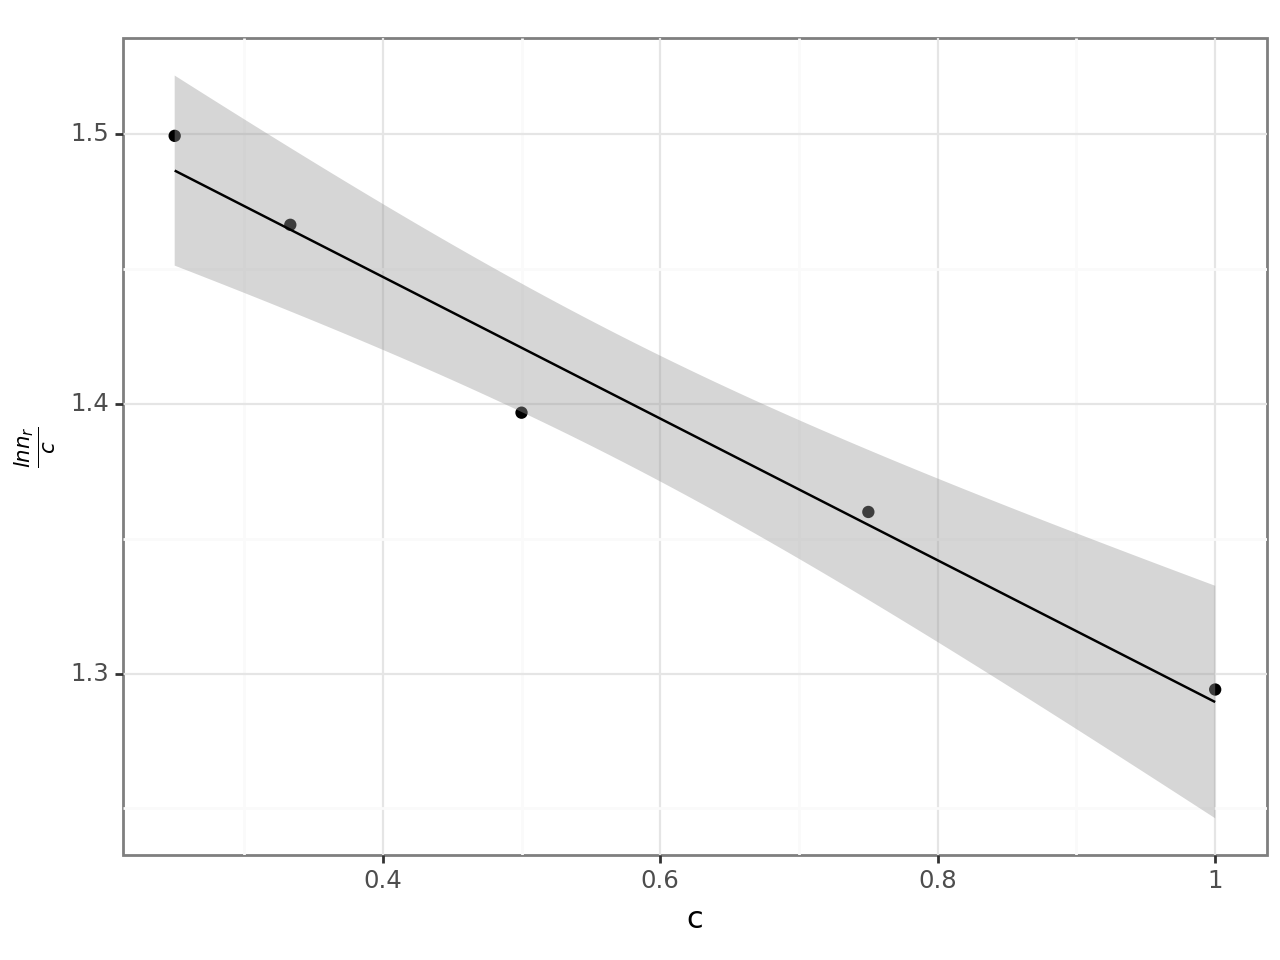
\includegraphics[scale = 0.1]{fig1.JPG} % 图片文件的名称和路径
  \caption{硝酸钾在水中的摩尔积分溶解热曲线}
  \label{fig:example}
\end{figure}

若将纯溶剂和纯溶质的摩尔焓分别表示为$H_m(1)$和$H_m(2)$,溶液中溶剂和溶质的偏摩尔焓分别表示为$H_{1,m}$和$H_{2,m}$,则恒压下将$n_2$量的溶质溶解于$n_1$量的溶剂时,过程的热效应

\[Q=\Delta H=n_1H_{1,m}+n_2H_{2,m}-[n_1H_m(1)+n_2H_m(2)]=n_1\Delta H_m(1)+n_2\Delta H_m(2)\]

式中Δ$H_m$(1)为摩尔微分稀释热,Δ$H_m$(2)为摩尔微分溶解热。

由摩尔积分溶解热的定义得
\[\Delta_{sol}H_m=\frac{\Delta H}{n_2}=\frac{n_1}{n_2}\Delta H_m(1)+\Delta H_m(2)=n_0\Delta H_m(1)+\Delta H_m(2)\]

在摩尔积分溶解热曲线图中,不同$n_0$点对应的切线斜率为该浓度下溶液的摩尔微分稀释热。即在上图中,A点对应浓度下的摩尔微分稀释热\[\left[ \frac{ \partial\Delta_{sol}H_m}{\partial n_0}\right] _{T,p,n_2} = \frac{AC}{BC}\]该切线在纵坐标上的截距OB即为对应于该浓度溶液的摩尔微分溶解热。

在含有1mol溶质的溶液中加入溶剂所产生的摩尔积分稀释热,就是两浓度下积分溶解热的差值。即在图2.1.2中,由A点相应浓度稀释至E点相应浓度,过程的摩尔积分稀释热$\Delta d_{il}H_m=EG-AF$

\section{实验步骤}
\subsection{仪器与试剂}
\begin{itemize}
    \item NDRH-2S型微机测定溶解热实验系统1套
    \item 计算机1台
    \item 最大称量为101g和610g的电子天平各1台
    \item 20x40mm称量瓶8个
    \item 毛笔1支
    \item 洗瓶1只
    \item 经研细与110℃烘干的硝酸钾(A.R.)
\end{itemize}

\subsection{操作流程}
\begin{enumerate}
    \item 依次在最大称量为101g的电子天平上准确称取2.5,1.5,2.5,3.0,3.5,4.0和4.5g$KNO_3$样品于已标号的称量瓶中。注意称量过程应盖上称量瓶盖子以防止样品吸潮,盛有样品的称量瓶应放人干燥器中备用。在最大称量为610g的电子天平上准确称取216.2g去离子水于干净干燥的保温杯中备用。
    \item 打开 NDRH-2S型微机测定溶解热实验系统电源,预热10min。
    \item 启动计算机至桌面状态。点击“溶解热数据测量系统”,进入系统界面,再点击“继续”,出现反应热测量系统界面,在上方的菜单栏点击“开始实验”,之后继续点击“开始实验”按钮,将干净、干燥的温度传感器置于空气中,此时系统开始自动测量室温。
    \item 待室温稳定后将温差置零,开启磁力搅拌器电源,调节磁力搅拌至中等速率,搅拌去离子水。根据计算机提示将加热装置连同温度传感器等一起置于保温杯内中的去离子水中,注意温度传感器探头不要与搅拌磁子和加热电热丝相接触。调节恒流电源,使加热器功率在2.25W到2.3W之间。此时体系开始升温。
    \item 当温度传感器采样到水温高于室温0.5℃时,计算机提示加入第一份$KNO_3$样品,加入后记录下加热器功率,同时计算机会实时记下此时水温和加热开始时间。加入$KNO_3$样品后,由于样品溶解吸热使水温下降,电热丝的加热使水温回升。当温度传感器探测到水温回升至第一份样品加入前的温度时,计算机提示加入第二份$KNO_3$样品,同时计算机给出第一份$KNO_3$样品溶解过程中的电热补偿通电时间。按计算机提示重复加样操作,直至加完8份$KNO_3$样品,计算机显示实验完成为止。注意,样品加入应少量连续,防止加样管被样品堵塞,每次加样后用毛笔将称量瓶和加样漏斗上残留的样品刷入加样孔。
    \item 加样结束后按计算机提示点击对话框右下方的“退出”按钮退出实验。将NDRH-2S型微机测定溶解热实验系统的电流调节旋钮调至零,停止搅拌并关闭搅拌器电源。在计算机菜单栏中点击“数据处理”按钮进入数据处理步骤,按计算机提示输入$KNO_3$和水的实际称量值与电热丝实际加热功率,点击“当前数据处理”按钮由计算机根据实际数据处理出本次实验结果,记录下计算机处理所得全部相关数据及实验结果。点击“下一页”可看到计算机画出的硝酸钾的摩尔积分溶解热曲线。
\end{enumerate}
\newpage
\section{数据记录}
    水的质量:216.3g  功率:2.320w 室温:23.82℃ 系统温度:24.32℃\\ 
\begin{table}[H]
    \centering
    \caption{数据记录表}
    \begin{tabular}{ccccccccc}
    \toprule
    & \multicolumn{8}{c}{序号} \\
    \cmidrule{2-9} 
    & 1 & 2 & 3 & 4 & 5 & 6 & 7 & 8 \\
    \midrule
    累计$KNO_3的质量$ & 2.49 & 3.99 & 6.49 & 9.5 & 12.99 & 16.89 & 20.85 & 25.32 \\
    $n_0$ & 487.4 & 304.2 & 187.0 & 127.8 & 93.4 & 71.9 & 58.2 & 27.9 \\
    累计加热时间(s)& 403.3 & 646.5 & 1052.6 & 1511.2 & 2003.9 & 2563.0 & 3116.8 & 3641.0 \\
    溶解热Q(J) & 940.3 & 1499.9 & 2442.0 & 3506.0 & 4649.0 & 5946.2 & 7231.0 & 8447.1 \\
    积分溶解热$Q_s$(kJ/mol) & 38.141 & 37.967 & 38.003 & 37.274 & 36.147 & 35.558 & 35.028 & 33.695 \\
    \bottomrule
    \end{tabular}
\end{table}

\section{数据处理与结果讨论}
\subsection{作出硝酸钾的摩尔积分溶解热曲线图}
\begin{figure}[H]
  \centering
  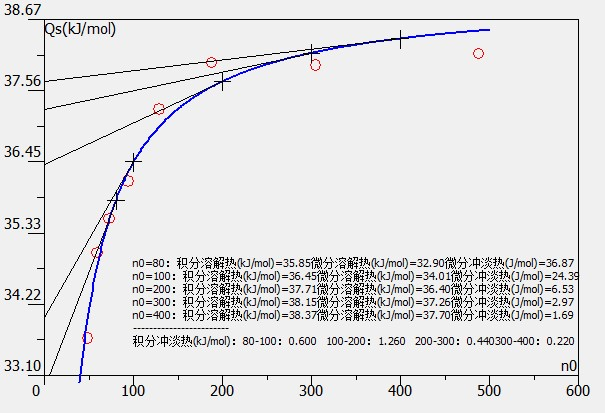
\includegraphics{1.jpg} 
  \caption{硝酸钾摩尔积分溶解热曲线}

\end{figure}

\subsection{结果分析与讨论}
从拟合后的曲线中我们可以发现,数据点存在不符合变化趋势的波动,说明实验中存在一定误差,原因可能如下:
\begin{enumerate}
    \item 我们观察到加热装置的功率并没有一直保持恒定,但是最后用于计算溶解热的功率软件默认为实验结束时的功率。实验开始时的功率为2.287w;当实验进行到第四组左右时,功率增加到2.309w;到第六组时,功率上升到2.318w。所以实际功率应当小于系统用于计算的功率,测得的$Q=W_{measure}t$, 相对误差$\delta = \frac{W_{measure}-W_{real}}{W_{real}} \times 100 \% $,溶解热Q的相对误差是随着$n_0$减小而变小的。这也可以解释前四组数据(图中后四组数据)波动较大,误差较大的原因。
    \item 加料的速度过慢可能导致温度波动较大,测量的时候传感器和软件具有滞后性,这样会导致测得的平衡点时间偏长,导致Q偏大。
    \item 硝酸钾容易吸潮,如果称量的时候样品中有水分,则每一组$n_0$都会偏大,带来误差。
    \item 实验开始前,若保温杯中若有残留水没有清理干净,那么会导致$n_0$偏小,带来误差。
\end{enumerate}

\subsection{注意事项}
\begin{enumerate}
    \item 由于硝酸钾容易吸潮,故样品应事先研细、烘干,置于干燥器中保存。称量过程应盖上称量瓶盖子以防止样品吸潮,盛有样品的称量瓶应放入干燥器中备用。
    \item 样品加入应少量连续,防止加样管被样品堵塞,加样后用毛笔将称残留的样品刷入加样孔。
    \item 实验前应确保实验用保温杯、加热装置、温度传感器等均处于干净、干燥的备用状态。
    \item 摩尔微分溶解热通过镜像法作切线求取。
\end{enumerate}


\section{思考题}
\subsection{本实脸装置是否适用于放热过程的热效应测定?}
可以,但是我认为结果误差会比较大,因为这套装置使用的是电热补偿法来进行热效应的测定,电热丝加热并不能使放热过程回到平衡温度。如要测定放热过程的热效应需要记录记录放热过程的最高温度,然后等待溶液降温到室温,在使用电补偿法加热到最高温度;不准确的原因是放热过程,比如说溶解热是需要时间的,在放热的过程中溶液浓度不均且也会和外界发生热交换,导致测得的最高温度可能并不准确。
\subsection{若实验开始设定为水温与室温相等时计算机提示加人第一份KNO,样品,则对实验结果是否会有影响?}
如果实验设计为在体系温度高于0.5℃时加入第一份硝酸钾样品,则可确保实验过程中高于室温和低于室温的时间大致相等。这样做可以使得从环境中吸收的热量和向外界释放的热量保持大致平衡,从而提高实验的准确性。

而如果在实验开始时即在水温与室温相等时加入第一份硝酸钾样品,可能会导致实验初期体系温度低于室温的时间较长。这会打破体系与环境间热量吸收与释放的平衡,可能影响实验结果的准确性。因此,为了提高实验的准确性,建议在体系温度高于室温0.5℃时再加入第一份硝酸钾样品。
\subsection{若实验结束后发现加样管中残留了一些 KNO,固体或 KNO,固体没有经过干燥处理,则这两种情况对实验结果有何影响?}
如果在测定溶解热的硝酸钾实验结束后发现加样管中残留了固体硝酸钾,这将影响实验结果的准确性。这是因为未完全溶解的固体硝酸钾意味着实际参与反应的硝酸钾质量小于预期,导致测得的溶解热偏低。

另一方面,如果硝酸钾固体没有经过干燥处理,可能含有一定量的水分。这将导致实际参与反应的硝酸钾质量小于预期,因为部分质量被水分占据。结果是测得的溶解热偏低。

因此,为了提高实验结果的准确性,建议在实验开始前确保固体硝酸钾已充分干燥,并在实验过程中确保所有固体硝酸钾能够完全溶解。
\subsection{如何获得反应 $CaCl_2(s)+6H_2O(l)\rightarrow CaCl_2\cdot 6H_2O(s)$的热效应?}
\begin{enumerate}
    \item 首先测定环境温度 T 并记录下来。然后设置系统温度为 T-0.5℃,记为 $T_0$。
    \item 加入一定量的固体$CaCl_2$到水中,观察温度变化,记录变化值为$\Delta T$。
    \item 等待系统温度恢复至$T_0$,确保温度稳定。
    \item 使用电补偿法测量从$T_0$到$T_0+\Delta T$所需的热量。
    \item 计算热效应。
    
\end{enumerate}
\end{document}






